\chapter{The ellipsoid method}
\label{el:cha:ellipsoid-method}


It is not known whether the  simplex algorithm is  an algorithm that
runs in polynomial 
time. For many pivoting rules it was even proved to require an
exponential number of iterations~\cite{MR0332165}.  It was long open, whether there exists a polynomial time
algorithm for linear programming until Khachiyan~\cite{Khachiyan79}
showed that the ellipsoid method\cite{Shor77,MR736268} can solve
linear programs in polynomial time. The remarkable fact is that the
algorithm is polynomial in the binary encoding length of the linear
program. In other words, if the input consists of the problem
$\max\{c^Tx\colon x \in \setR^n, \, Ax \leq b\}$, where $A\in \setQ^{m\times n}$ and $b
\in \setQ^m$, then the algorithm runs in polynomial time in $m+n+s$, where
$s$ is the largest binary encoding length of a rational number
appearing in $A$ or $b$. The question, whether there exists an
algorithm which runs in time polynomial in $m+n$ and performs
arithmetic operations on numbers, whose binary encoding length remains
polynomial in $m+n+s$ is one of the most prominent open problems in
theoretical computer science and discrete optimization.

Initially, the ellipsoid method can be used to solve the following
problem. 
\begin{quote}
  Given a matrix $A \in \setZ^{m\times n}$ and a vector $b \in \setZ^m$, determine a
  feasible point $x^*$ in the polyhedron $P = \{ x \in \setR^n \mid Ax\leq b\}$ or
  assert that $P$ is \emph{not full-dimensional} or $P$ is unbounded.   
\end{quote}
%
After we understand how the ellipsoid method solves this problem in
polynomial time, we discuss why linear programming can be solved in
polynomial time. 

Clearly, we can assume that $A$ has full column rank. Otherwise, we
can find with Gaussian elimination an invertible matrix $U \in
\setR^{n\times n}$ with $A \cdot U = \smat{A' & 0}$ where $A'$ has full column rank. The
system $A'x\leq b$ is then feasible if and only if $Ax\leq b$ is feasible. 

\begin{exercise}
  \label{el:ex:6}
  Let $x'$ be a feasible solution of $A'x\leq b$ and suppose that $U$ from
  above is given. Show how to compute a feasible solution $\tilde{x}$ of
  $Ax\leq b$. Also vice versa, show how to compute $x'$, if 
  $\tilde{x}$ is
  given. 
\end{exercise}

The \emph{unit ball} is the set $B = \{ x \in \setR^n \mid \|x\|\leq1\}$ and an
\emph{ellipsoid} $E(A,b)$ is the image of the unit ball under a linear map
$t:\setR^n\to\setR^n$ with $t(x) = Ax +b$, where $A \in \setR^{n\times n}$ is an invertible
matrix and $b \in \setR^n$ is a vector.  Clearly 
\begin{equation}
  \label{el:eq:113}
  E(A,b) =  \{ x \in \setR^n \mid \|  A^{-1} x - A^{-1} b \| \leq1\}. 
\end{equation}
%



\begin{exercise}
  \label{el:ex:8}
  Consider the mapping $t(x) = \smat{1 & 3 \\ 2 & 5}
  \smat{x_1\\x_2}$. Draw the ellipsoid which is defined by $t$. What
  are the axes of the ellipsoid? 
\end{exercise}


The \emph{volume} of the unit ball is denoted by $V_n$, where $V_n \sim
\frac{1}{\pi\,n} \left( \frac{2\,e\,\pi}{n}\right)^{n/2}$. It follows that
the volume of the ellipsoid $E(A,b)$ is equal to $|\det(A)| \cdot V_n$.
The next lemma is the key to the development of the ellipsoid method. 

\begin{lemma}[Half-Ball Lemma]
  \label{el:lem:12}
  The half-ball $H=\{x \in \setR^n \mid \|x\|\leq1, x_1\geq0\}$ is contained in the
  ellipsoid 
  \begin{equation}
    \label{el:eq:13}
    E = \left\{ x \in \setR^n \mid \left(\frac{n+1}{n}\right)^2  \left( x_1 -
      \frac{1}{n+1}\right)^2 + \frac{n^2-1}{n^2} \sum_{i=2}^n x_i^2 \leq1 \right\}
  \end{equation}
\end{lemma}



\begin{figure}[htbp]
  \centering 
  {
    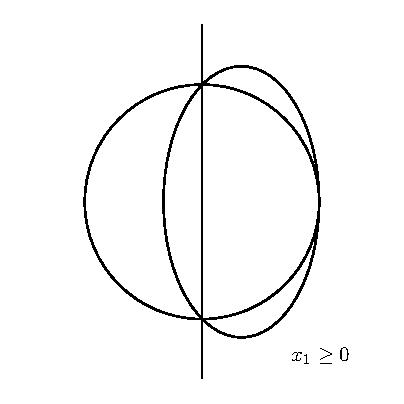
\includegraphics{figures/ellipsoid1.pdf}
  }
  \caption{Half-ball lemma.}
  \label{el:fig:half-ball}
\end{figure}


\begin{proof} 
  Let $x$ be contained in the unit ball, i.e., $\|x\|\leq1$ and suppose
  further that $0\leq x_1$ holds.  We need to show that 
  \begin{equation}
    \label{el:eq:16}
    \left(\frac{n+1}{n}\right)^2  \left( x_1 -
      \frac{1}{n+1}\right)^2 + \frac{n^2-1}{n^2} \sum_{i=2}^n x_i^2 \leq1 
  \end{equation}
  holds. 
  Since $\sum_{i=2}^nx_i^2\leq1 - x_1^2$ holds we have 
  \begin{equation}
    \label{el:eq:15}
    \begin{split}      
    \left(\frac{n+1}{n}\right)^2  \left( x_1 -
      \frac{1}{n+1}\right)^2 & + \frac{n^2-1}{n^2} \sum_{i=2}^n x_i^2 \\    
                            & \leq     \left(\frac{n+1}{n}\right)^2  \left( x_1 -
      \frac{1}{n+1}\right)^2 + \frac{n^2-1}{n^2} (1-x_1^2)     
  \end{split}
\end{equation}
This shows that~\eqref{el:eq:16} holds if $x$ is contained in the
half-ball and $x_1=0$ or $x_1=1$. Now consider the right-hand-side
of~\eqref{el:eq:15} as a function of $x_1$, i.e., consider 
\begin{equation}
  \label{el:eq:17}
  f(x_1) = \left(\frac{n+1}{n}\right)^2  \left( x_1 -
    \frac{1}{n+1}\right)^2 + \frac{n^2-1}{n^2} (1-x_1^2).    
\end{equation}
The first derivative is 
\begin{equation}
\label{el:eq:18}
  f'(x_1) = 2\cdot \left(\frac{n+1}{n}\right)^2  \left( x_1 -
    \frac{1}{n+1}\right) -  2\cdot \frac{n^2-1}{n^2} x_1.    
\end{equation}
We have $f'(0)<0$ and since both $f(0)=1$ and $f(1)=1$ (and since 
$f(x_1)$ is a 2-degree polynomial w.r.t. $x_1$),  we have
$f(x_1)\leq1$ for all $0\leq x_1\leq1$ and the assertion follows. 
\end{proof}



In terms of a matrix $A$ and a vector $b$, the ellipsoid $E$ is
described as $E = \{ x \in \setR^n \mid \| A^{-1} x - A^{-1}b\|\}$, where $A$
is the diagonal matrix with diagonal  entries
\begin{displaymath}
  \frac{n}{n+1},\sqrt{\frac{n^2}{n^2-1}},\ldots,\sqrt{\frac{n^2}{n^2-1}}
\end{displaymath}
and $b$ is the vector $b = (1/(n+1),0,\ldots,0)$. Our ellipsoid $E$ is thus
the image of the unit sphere under the linear transformation
$t(x)=Ax+b$. 
The determinant of $A$ 
is thus $\frac{n}{n+1}\left(\frac{n^2}{n^2-1}\right)^{(n-1)/2}$ which is
bounded by 
\begin{equation}
  \label{el:eq:19}
  e^{-1/(n+1)} e^{(n-1)/(2\cdot (n^2-1))} = e^{-\frac{1}{2(n+1)}}.  
\end{equation}
%
We can conclude the following theorem.
\begin{theorem}
  \label{el:thr:19}
  The half-ball $\{ x \in \setR^n \mid x_1\geq0, \, \|x\|\leq1\}$ is contained in an
  ellipsoid $E$, whose volume is bounded by $ e^{-\frac{1}{2(n+1)}} \cdot
  V_n$. 
\end{theorem}
%
% Consider now the unit-ball $B$ intersected with a half-space through
% the origin, thus the set 
% \begin{equation}
%   \label{el:eq:14}
%  H_c= B \cap (c^Tx\geq0) = \{ x \in \setR^n \mid \|x\|\leq1, \, c^Tx\geq0\}. 
% \end{equation}
% Clearly $H_c$ is the image of a \emph{rotation} $q(x) = Q\cdot x$, where
% $Q\in \setR^{n\times n}$ is an orthonormal matrix. The rotation  $q$ maps 
% $c^Tx\geq0$ to the half-space $x(1)\geq0$. Recall 
% that a matrix is called \emph{orthonormal} if $Q^TQ = I$. 
% \begin{exercise}
%   \label{el:ex:5}
%   Show that such a $Q$ exists. \emph{Hint: Recall the Gram-Schmidt
%     orthogonalization procedure and apply it to a basis of $\setR^n$ which
%     contains $c$}    
% \end{exercise}
% Since $H_c$ is the image of $H$ under the linear map $q(x)=Q\,x$ it
% follows from Theorem~\ref{el:thr:19} that $H_c$ is contained in the image
% of $E$ under the mapping $q$.  In fact, this is an ellipsoid, since it
% is the image of the unit sphere under the mapping $q\circ t$. 


Recall the following notion from linear algebra. A symmetric matrix $A
\in \setR^{n\times n}$ is called positive definite if all its eigenvalues are
positive.  Recall the following theorem. 
\begin{theorem}
  \label{el:thr:22}
  Let $A \in \setR^{n\times n}$ be a symmetric matrix. The following are
  equivalent. 
  \begin{enumerate}[i)]
  \item $A$ is positive definite. 
  \item $A = L^TL $, where $L\in \setR^{n\times n} $ is a uniquely determined upper
    triangular matrix. 
  \item $x^TAx>0$ for each $x \in \setR^n \setminus\{0\}$. 
  \item $A = Q^T \textrm{diag}(\lambda_1,\ldots,\lambda_n) Q$, where $Q \in \setR^{n\times n}$ is an
    orthogonal matrix and $\lambda_i \in \setR_{>0}$ for $i=1,\ldots,n$. 
  \end{enumerate}
\end{theorem}


It is now convenient to switch to a different representation of an
ellipsoid. An ellipsoid $\eE(A,a)$ is the set  $\eE(A,a) = \{ x \in \setR^n \mid
(x-a)^TA^{-1}(x-a)\leq 1\}$, where $A \in \setR^{n\times n}$ is a symmetric positive
definite matrix and $a\in \setR^n$ is a vector, called the 
\emph{center} of the ellipsoid.  Consider the half-ellipsoid
$\eE(A,a) \cap (c^Tx\leq c^Ta)$.

Our goal is a similar lemma as the half-ball-lemma for ellipsoids.
Geometrically it is clear that each half-ellipsoid $\eE(A,a) \cap
(c^Tx\leq c^Ta)$ must be contained in another ellipsoid $\eE(A',b')$
with $\vol(\eE(A',a'))/ \vol(\eE(A,a))\leq e^{-1/(2n)}$.  More precisely
this follows from the fact that the half-ellipsoid is the image of the
half-ball under a linear transformation. Therefore the image of the
ellipsoid $E$ under the same transformation contains the
half-ellipsoid.  Also, the volume-ratio of the two ellipsoids is
invariant under a linear transformation.


We now record the formula for the ellipsoid $\eE'(A',a')$. 
It is defined by 
\begin{eqnarray}
  \label{el:eq:20}
  a' &  = & a - \frac{1}{n+1}b \\
  A' & = & \frac{n^2}{n^2-1}\left( A - \frac{2}{n+1}b\, b^T   \right),
\end{eqnarray}
where $b$ is the vector $b = A\, c/ \sqrt{c^TA\,c} $.  
The proof of the correctness of this formula  can be found
in~\cite{GroetschelLovaszSchrijver88}.  
\begin{lemma}[Half-Ellipsoid-Theorem]
  \label{el:thr:20}
  The half-ellipsoid $\eE(A,b) \cap (c^Tx\leq c^Ta)$ is contained in the
  ellipsoid $\eE'(A',a')$ and one has $\vol(\eE')/
  \vol(\eE)\leq e^{-1/(2n)}$. 
\end{lemma}



%\begin{proof}
%  If $c^T$ is the vector $(-1,0,\ldots,0)$, and $a=0$, then 
%  \begin{eqnarray*}
%    b & = & (-1,0,\ldots,0)\\
%    a' &=& a - \frac{1}{n+1}b = (1/(n+1),0,\ldots,0)^T\\
%    A' &=& \diag\left(\frac{n^2}{(n+1)^2},\frac{n^2}{n^2-1}
%      ,\ldots,\frac{n^2}{n^2-1}\right) 
%  \end{eqnarray*}
%  and thus the assertion follows from Lemma~\ref{el:lem:12}.


%  We now denote the matrix
%  $\diag\left(\frac{n^2}{(n+1)^2},\frac{n^2}{n^2-1}
%    ,\ldots,\frac{n^2}{n^2-1}\right)$ by $D$ and the vector
%  $(1/(n+1),0,\ldots,0)^T$ by $d$.
% To this end, recall the notation from above, where $B$ denotes the
% unit ball and $E$ denotes the ellipsoid $\eE(D,d)$ which contains
% the half-ball $B \cap (x(1)\geq0)$.  

% Let $\eE(A,a)$ be any ellipsoid and let $\eE'(A',a')$ be the
% ellipsoid defined by~\eqref{el:eq:20} above. The matrix $A$ is
% positive definite and thus can be factored into $A = F^TF$
% Clearly there exists a \emph{rotation} or orthonormal matrix $Q$
% which maps $Fc$ to a positive multiple of $(-1,0,\ldots,0)^T$, i.e., with
%\begin{equation}
%  \label{el:eq:21}
%  (-1,0,\ldots,0)^T = Q F c/ \|Q F c\|. 
%\end{equation}
%The function
%\begin{equation}
%  \label{el:eq:22}
%  T(x) =  F Q^T x +a, 
%\end{equation}
%is a bijective affine transformation with
%$T^{-1}(x)=QF^{-1}(x-a)$.  
%One has
%\begin{eqnarray*}
%  T(B) & = & \{ T(y) \mid y^Ty\leq1\} \\
%       & = & \{ x \mid (T^{-1}(x))^T(T^{-1}(x))\leq1 \\
%       & = & \{ x \mid (x-a)^T (F^{-1})^TQQ^TF^{-1}\\
%       & = & \{ x \mid (x-a)^T A^{-1} (x-a)\leq1\}\\
%       & = & \eE.
%\end{eqnarray*}
%The image of $E$ under $T(x)$ is 
%\begin{eqnarray*}
% T(B) & = & \{ T(y) \mid (y-d)^TD^{-1} (y-d)\leq1\} \\
%       & = & \{ x \mid (T^{-1}(x)-d)^T D^{-1} (T^{-1}(y)-d)\leq1 \\
%       & = & \{ x \mid (x-d-a)^T (F^{-1})^TQDQ^TF^{-1}\\
%       & = & \{ x \mid (x-a)^T A^{-1} (x-a)\leq1\}\\
%       & = & \eE.
%\end{eqnarray*}
%\end{proof}

Before talking about the method, we give a useful definition.

\begin{definition}
   A polyhedron $P$ is full-dimensional if it has positive volume.
\end{definition}

\section{The method}
\label{el:sec:method}



Suppose  we know the following things of our polyhedron $P$. 
\begin{enumerate}[I)]
\item We have a number $L$ such that $\vol(P)\geq L$ if $P$ is
  full-dimensional.
\item We have an ellipsoid $\eE_{init}$ which contains $P$ if $P$ is
  bounded.
\end{enumerate}
The ellipsoid method is now easily described.


\begin{algorithm}[Ellipsoid method exact version]
\label{el:alg:3}
~

\begin{enumerate}[a)]
\item (Initialize): Set $\eE(A,a) := \eE_{init}$ \label{el:item:2}
\item If $a \in P$, then assert $P \neq \emptyset$ and stop  \label{el:item:1} 
\item If $\vol(\eE)<L$, then assert that $P$ is unbounded or $P$ is
  not full-dimensional \label{el:item:3}
\item Otherwise, compute an inequality $c^Tx\leq\beta$ which is valid for
  $P$ and satisfies $c^Ta>\beta$ and replace $\eE(A,a)$ by $\eE(A',a')$
  computed with formula~\eqref{el:eq:20} and goto
  step~\ref{el:item:1}).\label{el:item:4}  
\end{enumerate}
\end{algorithm}
%
\begin{theorem}
  \label{el:thr:21}
  The ellipsoid method computes a point in the polyhedron $P$ or
  asserts that $P$ is unbounded or not full-dimensional. The number of
  iterations is bounded by  $2\cdot n \ln (\vol(\eE_{init}) / L)$.
\end{theorem}


\begin{proof}
  Unless $P$ is unbounded, we start with an ellipsoid which contains
  $P$. This then holds for all the subsequently computed
  ellipsoids. After $i$ iterations one has
  \begin{equation}
    \label{el:eq:23}
    \vol(\eE)/ \vol(\eE_{init}) \leq e^{-\frac{i}{2n}}.
  \end{equation}
 Since we stop when $\vol(\eE)<L$, we stop at least after $2\cdot n
 \ln(\vol(\eE_{init})/ L)$ iterations. This shows the claim.   
\end{proof}



\section{Deciding feasibility}
\label{sec:deciding-feasibility}
Suppose that we have to decide the feasibility of $P = \{x ∈  ℝ^n : Ax ≤ b\}$
using the ellipsoid method described above. Here $A ∈ ℤ^{m ×n}$
and $b ∈ ℤ^{m}$.
In the following $B$
is an upper bound on the absolute values of the components of $A$
and $b$.

To apply the ellipsoid method we have to take care of the following items: 
\begin{enumerate}[i)]
\item We have to find a starting ball that contains a subset of the feasible region. \label{item:4}
\item We have to deal with the fact that $P$ might not be full dimensional even if it is feasible.  \label{item:7}
\item We have to bound the volume $P$ from below, if $P$ is full dimensional. \label{item:8}
\end{enumerate}


We first deal with the issue~\ref{item:4}). 
Suppose that there exists a feasible point $x^*$ and consider the index sets 
$I = \{ i : x^*_i ≥0 \}$ and $J = \{j : x^*_j ≥0\}$.    The polyhedron 
\begin{displaymath}
P' =   \{ x ∈ ℝ^n : Ax ≤b, x_i ≥ 0, i ∈ I, \, x_j ≤ 0, j ∈ J\}
\end{displaymath}
is contained in $P$ and it has vertices. Clearly $P'$ is described by a system of inequalities $Cx≤d$ where each component of $C$ and $d$ is bounded by $B$ in absolute value. 

A vertex $v^*$ of $P'$ is of the form $v^* = C_B^{-1} b_B$ for a basis $B$ of $C$. Since $C_B^{-1} = \widetilde{C_B} / \det(C_B)$ where $\widetilde{C_B} \in ℤ^{n ×n}$ is the adjoint of $C_B$. Each component of $\widetilde{C_B}$ is, by the Hadamard bound, bounded by $B^n ⋅ n^{n/2}$.  It follows that $\|v^*\|_∞$ is bounded by 
 $n^{n/2+1} ⋅ B^{n+1}$. We can thus conclude that $P$ is infeasible if and only if 
 \begin{displaymath}
   P ∩ \{ x ∈ ℝ^n : \|x\|_∞ ≤ n^{n/2+1} ⋅ B^{n+1} \}
 \end{displaymath}
is infeasible. 
For this polyhedron, we have a starting ellipsoid which is the ball of radius $n^{n/2+1} ⋅ B^{n+1} $ around $0$.  


Next, we deal with the issue~\ref{item:7}). 
\begin{exercise}
  \label{el:ex:11}
  Let $P = \{ x \in \setR^n \mid Ax\leq b\}$ be a polyhedron and $\varepsilon>0$ be a
  real number. Show that $P_\varepsilon = \{ x \in \setR^n \mid Ax\leq b+ \varepsilon\cdot
  \mathbf{1}\}$ is full-dimensional if $P \neq \emptyset$.
\end{exercise}


The above exercise raises the following question.  Is there an $\varepsilon>0$
such that $P_\varepsilon = \emptyset$ if and only if $P = \emptyset$ and furthermore is the
binary encoding length of this $\varepsilon$ polynomial in the binary encoding
length of $A$ and $b$? 

We recall the Farkas' lemma (Theorem~\ref{thr:7}). 
\begin{theorem}
  \label{el:thr:24}
  The system $Ax\leq b$ does not have a solution if and only if there
  exists a nonnegative vector $\lambda \in \setR^m_{\geq0}$ such that $\lambda^TA = 0$
  and $\lambda^Tb=-1$. 
\end{theorem}


%Again, suppose  $A\in \setZ^{m\times n}$ and $b\in \setZ^m$ and let $B$ be the largest absolute
%value of a coefficient of $A$ and $b$.  If $Ax\leq b$ is not feasible,
%then there exists a $\lambda\geq0$ such that $\lambda^T(A|b) = (\mathbf{0}|-1)$. 
If $Ax ≤b$ is infeasible, then the polyhedron 
\begin{displaymath}
  \{ λ ∈ ℝ^m : λ^TA = 0, \, λ^T b = -1 , \, λ ≥0 \} 
\end{displaymath}
has vertices. As we have argued before, there exists a vertex $λ^*$ of $P$ such that $\|λ^*\| ≤ n^{n/2+1} ⋅  B^{n+1}  $. 

Now let $\varepsilon =  (2 ⋅ m ⋅ n^{n/2+1} ⋅ B^{n+1})^{-1}$. Then $|{λ^*}^T \mathbf{1} \cdot \varepsilon |<1$ and thus 
\begin{equation}
  \label{el:eq:42}
  \lambda^T (b+ \varepsilon \cdot \mathbf{1}) <0. 
\end{equation}
%
Consequently the system $Ax\leq b+\varepsilon \cdot \mathbf{1}$ 
is infeasible if and only
if $Ax\leq b$ is infeasible. Furthermore, if $Ax\leq b+\varepsilon \cdot \mathbf{1}$  is feasible, then the polyhedron described by this set of inequalities is full-dimensional. 
Notice again that the encoding length of
$\varepsilon$ is polynomial in the encoding length of $Ax\leq b$.  % and we conclude
% with the main theorem of this section. 

% This discussion is summarized in the following lemma. 

% \begin{lemma}
%   \label{lem:2}
%   Let $A ∈ ℤ^{m ×n}$ and $b ∈ ℤ^m$ and let $B$ be an upper bound on the absolute value of the entries of $A$ and $b$ and let $K = (2 ⋅ m ⋅ n^{n/2+1} ⋅ B^{n+1})$. 
% Then $Ax ≤ b $ is feasible if and only of $ K ⋅ A x ≤ K ⋅ b + \mathbf{1}$ is feasible. The binary encoding length of $ K ⋅ A x ≤ K ⋅ b + \mathbf{1}$ is polynomial in the binary encoding length of $Ax ≤b$. 
% \end{lemma}

Next we deal with issue~\ref{item:8}.  We ask ourselves the following question. If $P = \{x ∈ ℝ^n : Ax ≤b\}$ is full-dimensional and bounded, what is a lower bound on $\vol(P)$? 

If $P$ is full-dimensional, then $P$ contains $n+1$ affinely independent vertices $v_1,\dots,v_{n+1}$, see Exercise~\ref{exercise:3}.  Each of these vertices is of the form $v_i = v_i'/q_i$, where $v_i' ∈ ℤ^n$ and $q_i$ is a $n×n$-sub-determinant of $A$. Consequently 
\begin{eqnarray*}
  \vol(P) & ≥ & (1/  ∏_{i=1}^{n+1} q_i) ⋅ \vol(\conv(v'_1,\dots,v'_{n+1})) \\
          & ≥ & (B^{n}⋅ n^{n/2} )^{-n}⋅ 1/n!,
\end{eqnarray*}where the last inequality follows from the Hadamard bound and Exercise~\ref{exercise:1} and Exercise~\ref{exercise:2}. 
A crude bound on $\vol(P)$ is thus $\vol(P) ≥ 1 / (B^{n^2} ⋅ n^{2⋅n^2})$. 


We can conclude with the following theorem. 

\begin{theorem}
  \label{thr:11}
  Let $Ax ≤ b$ be a system of linear inequalities with $A∈ℤ^{m×n}$ and $b∈ℤ^{m}$. Let $B$ be an upper bound on the absolute value of the entries of $A$ and $b$. The ellipsoid medthod can decide in time polynomial in $n,m$ and $\log B$ whether $Ax ≤ b$ is feasible. 
\end{theorem}


The next theorem follows from binary search. Its proof is an exercise. 



\begin{theorem}
\label{thr:12}
Let $\max\{c^Tx : x ∈ ℝ^n, \, Ax ≤b\}$ be a linear program with $A ∈ ℤ^{m×n}$, $b ∈ ℤ^{m}$, $c ∈ Ζ^{n}$.  Let $B$ be an upper bound on the absolute value of the entries of $A$ and $b$. The ellipsoid method finds an optimal solution of the linear program if one exists in time polynomial in $n,m$ and $\log B$. 
  Let $Ax ≤ b$ be a system of linear inequalities with $A∈ℤ^{m×n}$ and $b∈ℤ^{m}$. Let $B$ be an upper bound on the absolute value of the entries of $A$ and $b$. The ellipsoid can decide in time polynomial in $n,m$ and $\log B$ whether $Ax ≤ b$ is feasible. 
\end{theorem}


\subsection*{Exercises} 

\begin{enumerate}
\item Show the following. If $P⊆ℝ^n$ is a bounded and full-dimensional polyhedron, then there exist vertices $v_1,\dots,v_{n+1}$ of $P$ that are affinely independent, i.e., $v_2-v_1, v_3-v_1, \dots, v_{n+1}-v_1$ are linearly independent. \emph{Hint: If $a^Tx = β$ is some hyperplane, where $a ∈ ℝ^n \setminus \{0\}$, then there exists a vertex of $P$ that is not contained in that hyperplane.}\label{exercise:3}
\item Show that $\vol(\conv(0,e_1,\dots,e_n)) = 1/n!$ \label{exercise:1}
\item Let $a_1,\dots,a_n ∈ℤ^n$ be linearly independent. Show that
  \begin{displaymath}
    \vol(\conv(0,a_1,\dots,a_n)) = |\det(a_1,\dots,a_n)| /n!. 
  \end{displaymath} \label{exercise:2}
\end{enumerate}

\section{The separation problem}
\label{el:sec:separation-problem}

At this point we can already notice a very important fact. Inspect
step~\ref{el:item:4} of the algorithm. What is required here? An
inequality which is valid for $P$ but not for the center $a$ of
$\eE(A,a)$. Such an inequality is readily at hand if we have the
complete inequality description of $P$ in terms of a system
$Cx\leq d$. Just pick an inequality which is violated by $a$. Sometimes
however, it is not possible to describe the polyhedron of a
combinatorial optimization problem with an inequality system
efficiently, simply 
because the number of inequalities is too large.
An example of such a polyhedron is the matching polytope, see
Theorem~\ref{po:thr:18}. 

The great power of the ellipsoid method lies in the fact that we do
not have to \emph{write down} the polyhedron entirely. We only have to
solve the so-called separation problem for the polyhedron, which is
defined as follows. 

\fancybox[Separation Problem]{ Given a
  point $a \in \setR^n$ determine, whether $a\in P$ and if not, compute an
  inequality $c^Tx\leq\beta$ which is valid for $P$ with $c^Ta>\beta$. }



\begin{exercise}
  \label{el:ex:10}
  We are given an undirected graph $G=(V,E)$. A \emph{spanning tree}
  $T$ is a subset $T\subseteq E$ of the edges such that $T$ does not contain
  a cycle and $T$ connects all the vertices $V$. Consider the
  following \emph{spanning tree polytope} $P_{span}$
\begin{eqnarray}
 \sum_{e\in E} x(e)       & = & n-1  \label{el:eq:26}\\
 \sum_{e\in \delta(U)} x(e)   & \geq & 1  \quad \quad \forall \emptyset \subset U \subset V  \label{el:eq:25}\\
                 x(e)  & \leq & 1 \quad \quad  \forall e\in E \\
                 x(e)  & \geq & 0 \quad \quad  \forall e\in E. 
\end{eqnarray}

Let $x$ be an integral solution of $P_{span}$ and define $T=\{e\in E \mid
x(e)=1\}$. The inequality~\eqref{el:eq:26} ensures that exactly $n-1$ edges are
picked. The  inequalities~\eqref{el:eq:25} ensure that $T$ connects the
vertices 
of $G$.  Thus $T$ must be a spanning tree.  Clearly, there are
exponentially many inequalities of type~\eqref{el:eq:25}.  Nevertheless,
a fractional solution of this polytope can be computed using the
ellipsoid method.

Show that the separation problem for $P_{span}$ can be solved in
polynomial time. 

\emph{Hint:} To verify whether a vector $x\in \setR_{\geq0}^{|E|}$ fulfills
inequalities of type~\eqref{el:eq:25}, it is a good idea to recall the
MinCut or MaxFlow problem.

{\small 
\noindent 
Via binary search even an optimal solution can be computed in
polynomial time (in the input length) if we introduce edge costs (you
don't have to show that). In the next semester you will see that any
optimal basis solution is integral and hence defines an optimal
spanning tree w.r.t. the edge costs.
}
\end{exercise}

\begin{exercise}
  \label{el:ex:7}
  Consider the triangle defined by
  \begin{eqnarray*}
    -x_1-x_2 & \leq & -2 \\
    3 x_1     & \leq & 4\\
    -2x_1 + 2x_2 & \leq & 3.
  \end{eqnarray*}
  
  Draw the triangle and simulate the ellipsoid method with starting
  ellipsoid being the ball of radius $6$ around $0$. Draw each of the
  computed ellipsoids with your favorite program (pstrics, maple,\ldots ).
  How many iterations does the ellipsoid method take?

  \emph{Ignore the occurring rounding errors!} 
\end{exercise}

% \section{How to start and when to stop }
% \label{el:sec:how-start-when-1}

% In our description of the ellipsoid method, we did not explain yet what
% the initial ellipsoid  is and when we can stop with asserting
% that $P$ is either not full-dimensional or unbounded. 


% Suppose therefore that $P = \{ x \in \setR^n \mid Ax\leq b\}$ is
% full-dimensional and bounded with $A\in \setZ^{m\times n}$ and $b\in \setZ^m$. Let
% $B$ be the largest absolute value of a component of $A$ and $b$. In this 
% section we will show the following things.  
% \begin{enumerate}[i)]
% \item The vertices of $P$ are in the box 
% $\{x \in \setR^n \mid -n^{n/2} B^n \leq x_i \leq n^{n/2} B^n$ 
% $\forall 1 \leq i \leq n \}$. 
% Thus $P$ is contained in the ball around $0$
%   with radius $n^{n} B^n$ . Observe that the encoding length of this
%   radius is $\size(n^{n}B^n) = O(n \log n + n\size(B))$ which is
%   polynomial in the dimension $n$ and the largest encoding length of a
%   coefficient of $A$ and $b$. \label{el:item:7}
% \item The volume of $P$ is bounded from below by  $1 /
% (n\cdot B)^{3n^2}$. \label{el:item:8}
% \end{enumerate}

% The following lemma is proved in any linear algebra course. 
% \begin{lemma}[Inverse formula and Cramer's rule]
%   \label{el:lem:11}
%   Let $C \in \setR^{n\times n}$ be a nonsingular matrix. Then 
%   \begin{displaymath}
%     C^{-1}(j,i) = (-1)^{i+j} \det(C_{ij}) / \det(C),
%   \end{displaymath}
%   where $C_{ij}$ is the matrix arising from $C$ by the deletion of the
%   $i^{th}$ row and $j^{th}$ column. If $d\in \setR^n$ is a vector 
%   then the $j^{th}$ component of $C^{-1}d$ is given by
%   $\det(\wt{C})/\det(C)$, where $\wt{C}$ arises from $C$ be 
%   replacing the $j^{th}$ column with $d$. 
%  \end{lemma}

% We now define the size of a rational number $r = p/q$ with $p$ and $q$
% relatively prime integers, a vector $c \in \setQ^n$ and a matrix $A \in
% \setQ^{m\times n}$: 
% \begin{itemize}
% \item $\size(r) = 1 + \lceil\log ( |p|+1) \rceil + \lceil \log( |q|+1) \rceil$
% \item $\size(c) = n+ \sum_{i=1}^n \size(c_i)$
% \item $\size(A) = m\cdot n + \sum_{i=1}^n\sum_{j=1}^m \size(A(i,j))$
% \end{itemize}



% We recall the Hadamard inequality which states that for $A \in
% \setR^{n\times n}$ one has 
% \begin{equation}
%   \label{el:eq:10}
%   |\det(A)| \leq \prod_{i=1}^n \|a_i\|,
% \end{equation}
% where $a_i$ denotes the $i^{th}$ column of $A$.  In particular, if $B$
% is the largest absolute value of an entry in $A$, then 
% \begin{equation}
%   \label{el:eq:11}
%   |\det(A)| \leq n^{n/2} B^{n}. 
% \end{equation}


% %\begin{exercise}[Computing the determinant with modular arithmetic]
% %  \label{el:ex:9}
% %  In this exercise we show how to compute the determinant of a matrix
% %  $A \in \setZ{n\times n}$ in polynomial time. We are all aware of the fact that
% %  Gaussian elimination performs $O(n^3)$ 
% %  \emph{arithmetic operations} to compute an upper triangular matrix
% %  $R \in \setQ^{n\times n}$ from $A$ such that $\det(R) = \det(A)$ and $\det(A)
% %  = \prod_{i=1}^n r(i,i,)$. But could the number of \emph{bits} which are
% %  necessary to represent the intermediate steps in Gaussian
% %  elimination explode~? We do not want to answer this question in this
% %  exercise. Instead we circumvent it by using the Hadamard
% %  inequality.   
% %\end{exercise}

% Now let us inspect the vertices of a polyhedron $P = \{ x \in \setR^n \mid
% Ax\leq b\}$, where $A$ and $b$ are integral and the largest absolute
% value of any entry in $A$ and $b$ is bounded by $B$. A vertex is
% determined as the unique solution of a linear system $A'x=b'$, where
% $A'x\leq b'$ is a subsystem of $Ax\leq b$ and $A'$ is invertible. Using
% Cramer's rule and our observation~\eqref{el:eq:11} we see that the
% vertices of $P$ lie in the box $\{x \in \setR^n \mid -n^{n/2} B^n \leq x_i \leq n^{n/2} B^n,$ $i = 1,\cdots,n\}$.  This
% shows~\ref{el:item:7}).


% Now let us consider a lower bound on the volume of $P$. Since $P$ is
% full-dimensional, there exist $n+1$ affinely independent vertices
% $v_0,\ldots,v_n$ of $P$ which span a \emph{simplex} in $\setR^{n}$ 
% (i.e. the $n$-dimensional polytope equivalent to the convex-hull of 
% these $n+1$ vertices). The
% volume of this simplex is determined by the formula
% \begin{equation}
%   \label{el:eq:24}
%   \frac{1}{n!} \cdot \left|\det \mat{1 & \cdots & 1 \\ v_0& \ldots&v_n} \right|. 
% \end{equation}
% %
% By Cramer's rule and the Hadamard inequality, the common  denominator
% of each component of $v_i$ can be  bounded by $n^{n/2} B^n$. Thus
% \eqref{el:eq:24} is bounded by 
% \begin{equation}
%   \label{el:eq:44}
%   1 / \left(   n^n (n^{\frac{n}{2}} \cdot B^n)^{n+1}      \right) \geq  1 /
%   \left(   n^{3n^2}   B^{2n^2}      \right) \geq 1 / (n\cdot B)^{3\cdot n^2},
% \end{equation}
% which shows \ref{el:item:8}). 


% Now we plug these values into our analysis in
% Theorem~\ref{el:thr:21}. Our initial volume $\vol(\eE_{init})$  is bounded by   the
% volume of the box with side-lengths $2 (n\cdot B)^n$. Thus
% \begin{equation}
%   \label{el:eq:27}
%   \vol(\eE_{init}) \leq(2\cdot n\cdot B)^{n^2}.  
% \end{equation}
% %
% Above we have shown that 
% \begin{equation}
%   \label{el:eq:38}
%   L \geq 1 / (n\cdot B)^{3n^2}. 
% \end{equation}
% Clearly 
% \begin{equation}
%   \label{el:eq:39}
%    \vol(\eE_{init}) / L  \leq 2^{n^2} \cdot (n \cdot B)^{4 \cdot n^2} 
%    \leq (2n \cdot B)^{4\cdot n^2}. 
% \end{equation}
% %
% By Theorem~\ref{el:thr:21} the ellipsoid method performs 
% \begin{equation}
%   \label{el:eq:40}
%   O\left(2\cdot n \cdot \ln \left((2n \cdot B)^{4\cdot n^2}\right) \right)
% \end{equation}
% iterations. This is bounded by 
% \begin{equation}
%   \label{el:eq:41}
%   O(n^3 \cdot \ln (n \cdot B)).
% \end{equation}
% Now recall that $\log B$ is the number of \emph{bits}  which are
% needed to encode the coefficient with the largest absolute value of
% the constraint system $Ax\leq b$ and that $n$ is the number of variables
% of this system. Therefore the expression~\eqref{el:eq:41} is polynomial
% in the binary input encoding of the system $Ax\leq b$. We conclude the
% following theorem. 

% \begin{theorem}
%   \label{el:thr:23}
%   The ellipsoid method (exact version)  performs a polynomial number
%   of iterations.  
% \end{theorem}




% \section{The boundedness and full-dimensionality condition}
% \label{el:sec:bound-full-dimens}



% In this section we want to show how the ellipsoid method can be used
% to solve the following problem. 
% \begin{quote}
%   Given a matrix $A \in \setZ^{m\times n}$ and a vector $b \in \setZ^m$, determine a
%   feasible point $x^*$ in the polyhedron $P = \{ x \in \setR^n \mid Ax\leq b\}$ or
%   assert that $P = \emptyset$. 
% \end{quote}
% %
% \subsection{Boundedness}
% \label{el:sec:boundedness}

% We have argued that the matrix $A \in \setZ^{m\times n}$ can be assumed to have
% full column rank. So, if $P$ is not empty, then $P$ does have at least
% one vertex. The vertices are contained in the box $\{x \in \setR^n \mid
% -n^{n/2} B^n \leq x_i \leq n^{n/2} B^n,$ $i=1,\cdots,n\}$. Therefore, we can append the
% inequalities $-n^{n/2} B^n \leq x_i \leq n^{n/2} B^n$ 
% $(i=1,\cdots,n)$ to $Ax\leq b$ without
% changing the status of $P \neq \emptyset$ or $P = \emptyset$. Notice that the
% \emph{binary encoding length} of the new inequalities is polynomial in
% the binary encoding length of the old inequalities.



% \begin{theorem}
%   \label{el:thr:25}
%   The ellipsoid method can be used to decide whether a system of
%   inequalities $Ax\leq b$ contains a feasible point, where $A\in\setZ^{m\times n}$
%   and $b\in \setZ^m$. The number of iterations is bounded by a polynomial
%   in $n$ and $\log B$, where $B$ is the largest absolute value of a
%   coefficient of $A$ and $b$.
% \end{theorem}

\section{The ellipsoid method for optimization}
\label{el:sec:ellips-meth-optim}

Suppose that you want to solve a linear program 
\begin{equation}
  \label{el:eq:43}
  \max \{ c^Tx \mid x \in \setR^n, \, Ax\leq b\} 
\end{equation}
and recall that if~\eqref{el:eq:43} is bounded and feasible, then so is
its dual and the two objective values are equal. Thus, we can use the
ellipsoid method to find a point $(x,y)$  with $c^Tx = b^Ty$, $Ax\leq b$
and $A^Ty=c, y\geq0$. 


However, we mentioned that the strength of the ellipsoid method lies
in the fact that we do not need to write the system $Ax\leq b$ down
explicitly. The only thing which has to be solvable is the
\emph{separation problem}. This is to be exploited in the next
exercise. 


\begin{exercise}
  \label{el:ex:12}
  Show how to solve the optimization problem $\max\{c^Tx \mid Ax\leq b\}$
  with a polynomial number of calls to an algorithm which solves the
  separation problem for $Ax\leq b$. You may assume that $A$ has full
  column rank and the polynomial bound on the number of calls to the
  algorithm to    solve the separation problem can depend on $n$ and
  the largest size of a component of $A,b$ and $c$. 
\end{exercise}


\section{Numerical issues}
\label{el:sec:numerical-issues}

We did not discuss the numerical details on how to implement the
ellipsoid method such that it runs in polynomial time. One issue is
crucial. 

\fancybox[!]{We only want to compute with a precision which is  polynomial in the input encoding! }


 In the formula~\eqref{el:eq:20} the vector $b$ is defined by
 taking a square root. The question thus rises on how to round the
 numbers in the intermediate ellipsoids such that they can be handled
 on a machine.  Also one has to analyze the growth of the numbers in
 the course of the algorithm. All these issues  can be overcome but we
 do not discuss them in this course. I would like to refer you to the
 book of Alexander Schrijver~\cite{Schrijver86}  for further
 details. They are not difficult, but a little technical. 




%\bibliographystyle{abbrv}

%\bibliography{mybib,papers,books,my_publications}


%%% Local Variables: 
%%% mode: latex
%%% TeX-master: "lecture"
%%% End: 
